
\subsection{Experiment Environment}
The experiments in this paper are conducted on Google Colab\cite{google_colab} with 1 CPU, 12GB RAM, and an NVIDIA GeForce T4 graphics card.
The main libraries used in this experiment includes nltk, pytorch, scikit-learn, transformers and matplotlib libraries.
For the code related to this experiment, please refer to the following link.\footnote{Source Code:https://github.com/qqyfly/text\_mining\_project} 

\subsection{Experiment Results}

In this experiment, we employed the BERT model for training and monitored the loss and accuracy, 
as illustrated in Figure 3. The plotted results indicate that the training loss consistently 
decreased from 0.14 to 0.02. Meanwhile, the validation loss exhibited a decreasing trend 
from approximately 0.1 to 0.07, albeit with fluctuations. However, after 12 epochs, 
an increase in the validation loss was observed, suggesting potential overfitting.

For the Accuracy, training accuracy increased from 0.94 to 0.99, while the validation accuracy
increased from around 0.964, and reached around 0.98, but still with some fluctuations
when epoches increasing. Over all, the BERT model archive a pretty good performance in this experiment.

% add a plot here
\begin{figure}[t]    
    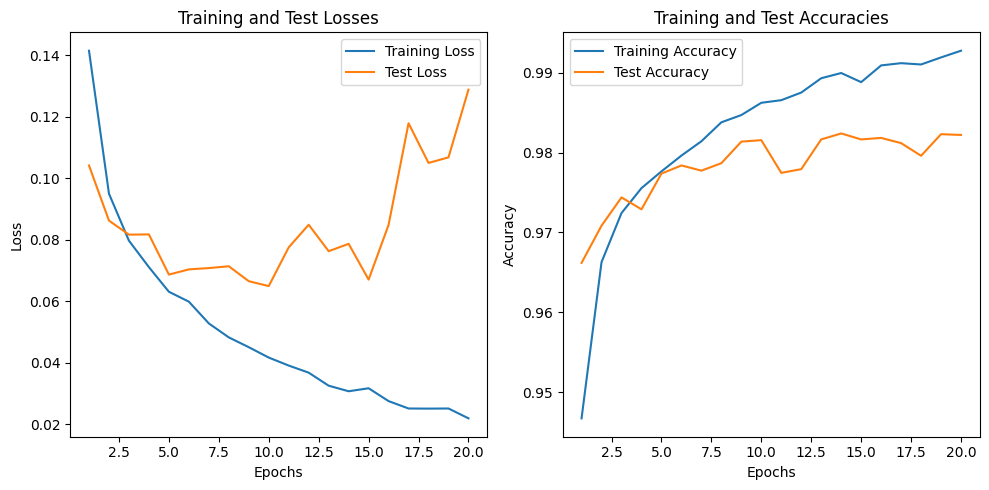
\includegraphics[width=1\linewidth]{figure/bert.png} \hfill
    \caption{BERT model Loss and Accuracy}
\end{figure}

For the GPT2 model, we notice that the accuracy is pretty low(around 0.55) compare to the BERT model(around 0.98), regarding the
loss value, it is drop to 0 after 2 epochs.

\begin{figure}[t]    
    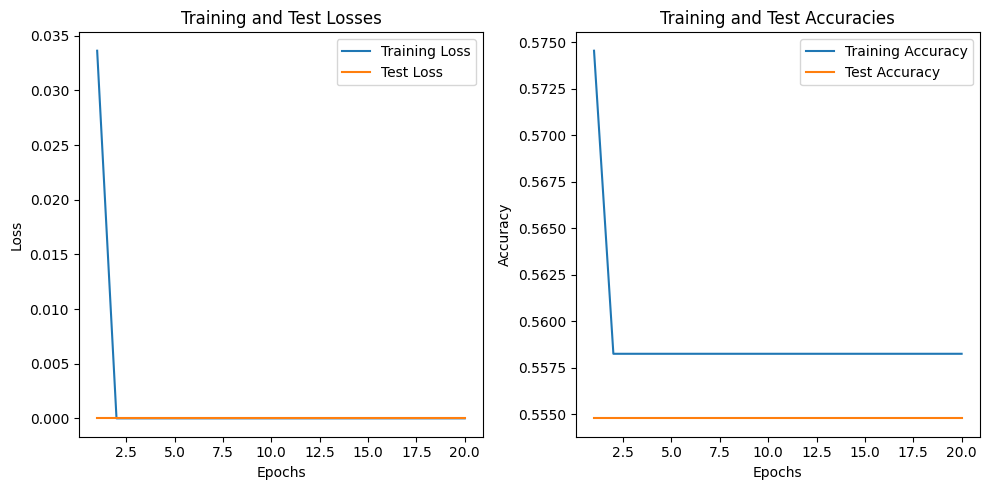
\includegraphics[width=1\linewidth]{figure/gpt.png} \hfill
    \caption{GPT model Loss and Accuracy}
\end{figure}

We list the final four values of the BERT and GPT2 models in Table 1.

%add a table here
\begin{table}
    \centering 
    \begin{tabular}{|c|c|c|}
        \hline
        \textbf{Model} & \textbf{BERT} & \textbf{GPT2} \\
        \hline
        Accuracy & 0.97987 & 0.44522\\
        \hline
        Precision & 0.97928 & 0\\
        \hline
        Recall & 0.98455 & 0\\
        \hline
        F1-score & 0.97987  & 0.27431\\
        \hline
    \end{tabular}
    \caption{BERT and GPT model evaluation}
\end{table}



